%NEURAL PRESY ;)

%----------------------------------------------------------------------------------------
%   PACKAGES AND THEMES
%----------------------------------------------------------------------------------------

\documentclass{beamer}

\mode<presentation> {

% The Beamer class comes with a number of default slide themes
% which change the colors and layouts of slides. Below this is a list
% of all the themes, uncomment each in turn to see what they look like.

%\usetheme{default}
%\usetheme{AnnArbor}
%\usetheme{Antibes}
%\usetheme{Bergen}
\usetheme{Berkeley}
%\usetheme{Berlin}
%\usetheme{Boadilla}
%\usetheme{CambridgeUS}
%\usetheme{Copenhagen}
%\usetheme{Darmstadt}
%\usetheme{Dresden}
%\usetheme{Frankfurt}
%\usetheme{Goettingen}
%\usetheme{Hannover}
%\usetheme{Ilmenau}
%\usetheme{JuanLesPins}
%\usetheme{Luebeck}
%\usetheme{Madrid}
%\usetheme{Malmoe}
%\usetheme{Marburg}
%\usetheme{Montpellier}
%\usetheme{PaloAlto}
%\usetheme{Pittsburgh}
%\usetheme{Rochester}
%\usetheme{Singapore}
%\usetheme{Szeged}
%\usetheme{Warsaw}

% As well as themes, the Beamer class has a number of color themes
% for any slide theme. Uncomment each of these in turn to see how it
% changes the colors of your current slide theme.

%\usecolortheme{albatross}
%\usecolortheme{beaver}
%\usecolortheme{beetle}
%\usecolortheme{crane}
%\usecolortheme{dolphin}
%\usecolortheme{dove}
%\usecolortheme{fly}
%\usecolortheme{lily}
%\usecolortheme{orchid}
%\usecolortheme{rose}
%\usecolortheme{seagull}
%\usecolortheme{seahorse}
%\usecolortheme{whale}
%\usecolortheme{wolverine}

%\setbeamertemplate{footline} % To remove the footer line in all slides uncomment this line
%\setbeamertemplate{footline}[page number] % To replace the footer line in all slides with a simple slide count uncomment this line

\setbeamertemplate{navigation symbols}{} % To remove the navigation symbols from the bottom of all slides uncomment this line
}

\usepackage{graphicx} % Allows including images
\graphicspath{ {images/} }
\usepackage{booktabs} % Allows the use of \toprule, \midrule and \bottomrule in tables
\usepackage{caption}
\usepackage{subcaption}
\usepackage{algorithm,algorithmic}
\usepackage{pgfplots}

\def\layersep{2cm}
\def\nodesep{0.25cm}
\usepackage{tikz}

%----------------------------------------------------------------------------------------
%   TITLE PAGE
%----------------------------------------------------------------------------------------

\title[Neural Networks Pt. 2]{Neural Networks Workshop: Training and Stochastic Gradient Descent}

\author[W.\,Guss \& P.\,Kuznetsov]
{%
  \texorpdfstring{
    \begin{columns}%[onlytextwidth]
      \column{.45\linewidth}
      \centering
      William Guss\\
      \href{mailto:wguss@berkeley.edu}{wguss@berkeley.edu}
      \column{.45\linewidth}
      \centering
      Phillip Kuznetsov\\
      \href{mailto:philkuz@berkeley.edu}{philkuz@berkeley.edu}
    \end{columns}
  }
  {William Guss \& Phillip Kuznetsov}
}
\institute[UCB]
{
University of California, Berkeley \\
Robotics @ Berkeley \\
}

\date{December 1, 2015} % Date, can be changed to a custom date
\makeatletter
\newcommand{\verbatimfont}[1]{\renewcommand{\verbatim@font}{\ttfamily#1}}
\makeatother
\begin{document}

\begin{frame}
\titlepage
\end{frame}

\begin{frame}

\begin{center}
\Huge Today we use and train Feed-Forward Artificial Neural Networks
\end{center}

\frametitle{Overview}
\tableofcontents
\end{frame}

%----------------------------------------------------------------------------------------
%   PRESENTATION SLIDES
%----------------------------------------------------------------------------------------

%------------------------------------------------
\section{Feed-Forward Neural Networks} % Sections can be created in order to organize your presentation into discrete blocks, all sections and subsections are automatically printed in the table of contents as an overview of the talk
%-----------------------------------------------

    \begin{frame}
        \frametitle{Perceptron Review}
        \begin{center}
            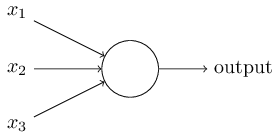
\includegraphics[scale=.3]{perceptron}
        \end{center}
        \begin{itemize}
        \item Perceptrons are neural computation units which make \emph{weighted} decisions:
        \begin{equation*}
            \begin{aligned}
                p(\pmb x) &= \left\{
                 \begin{array}l
                 1\ \text{if}\ \sum w_ix_i + b\geq 0\\
                 0\ \text{otherwise}
                \end{array}
                \right. \\
                &= \text{step}\left(\sum w_ix_i + b\right)
            \end{aligned}
        \end{equation*}
        \item Single perceptrons are not powerful enough, as seen last time with XOR.
        \item What if we want real valued output for tasks like predicting
         the temparature or stock prices?
        \end{itemize}
    \end{frame}

    \begin{frame}
        \frametitle{Feedforward Neural Networks}
        \begin{figure}
        \centering
        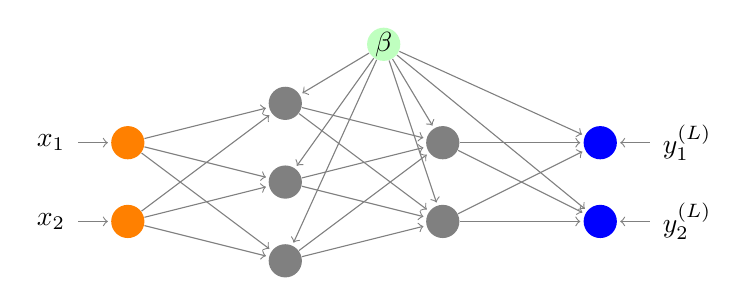
\begin{tikzpicture}[shorten >=1pt,->,draw=black!50, node distance=\layersep]
            \tikzstyle{every pin edge}=[<-,shorten <=1pt]
            \tikzstyle{neuron}=[circle,fill=black!25,minimum size=12pt,inner sep=0pt]
            \tikzstyle{input neuron}=[neuron, fill=orange];
            \tikzstyle{output neuron}=[neuron, fill=blue!100];
            \tikzstyle{hidden neuron}=[neuron, fill=black!50];
            \tikzstyle{annot} = [text width=3em, text centered]

           \node[hidden neuron, fill=green!25] (BIAS) at (3.25,0) {$\beta$};

            % Draw the input layer nodes
            \foreach \name / \y in {1,...,2}
            % This is the same as writing \foreach \name / \y in {1/1,2/2,3/3,4/4}
                \path[yshift=\nodesep]
                    node[input neuron, pin=left: \(x_\y\)] (I-\name) at (0,-0.5 cm -\y  cm) {};

            % Draw the hidden layer nodes
            \foreach \name / \y in {1,...,3}
                \path[yshift=\nodesep]
                    node[hidden neuron] (H1-\name) at (\layersep,-\y) {};

             \foreach \name / \y in {1,...,2}
                \path[yshift=\nodesep]
                    node[hidden neuron] (H2-\name) at (2*\layersep,-0.5cm -\y cm) {};

            % Draw the hidden layer nodes
            \foreach \name / \y in {1,...,2}
                \path[yshift=\nodesep]
                    node[output neuron, pin=right:\(y_{\name}^{(L)}\)] (O-\name) at (3*\layersep,-0.5cm -\y cm) {};


            % Connect every node in the input layer with every node in the
            % hidden layer.
            \foreach \source in {1,...,2}
                \foreach \dest in {1,...,3}
                    \path (I-\source) edge (H1-\dest);

            % Connect every node in the hidden layer with the output layer

            \foreach \source in {1,...,3}
                \foreach \dest in {1,...,2}
                    \path (H1-\source) edge (H2-\dest);
            \foreach \source in {1,...,2}
                \foreach \dest in {1,...,2}
                \path (H2-\source) edge (O-\dest);

              %Connect the bias
                \foreach \dest in {1,...,3}
                    \path (BIAS) edge (H1-\dest);
                \foreach \dest in {1,...,2}
                    \path (BIAS) edge (H2-\dest);
                \foreach \dest in {1,...,2}
                    \path (BIAS) edge (O-\dest);

            % Annotate the layers
        \end{tikzpicture}
        %   \caption[An example of a feed-forward ANN]{An example of a feed-forward ANN,  \(\mathcal{N}\) with four layers.}
        \end{figure}
        \begin{itemize}
        \item Feedforward Artifical Neural Networks (ANNs) are the \emph{continuous}
        extensions of perceptrons.
        \item ANNs can have many layers and different nodes
         which are \emph{fully connected.}

         \item The intuition behind this model is that each neuron in the network
         makes a weighted decision like the perceptron. Many \emph{stacked} decisions
         allows for extremely complex logic.
        \end{itemize}
    \end{frame}

    \subsection{How It Works} % A subsection can be created just before a set of slides with a common theme to further break down your presentation into chunks
    \begin{frame}
        \frametitle{A Bit of Notation}
             \begin{figure}
        \centering
        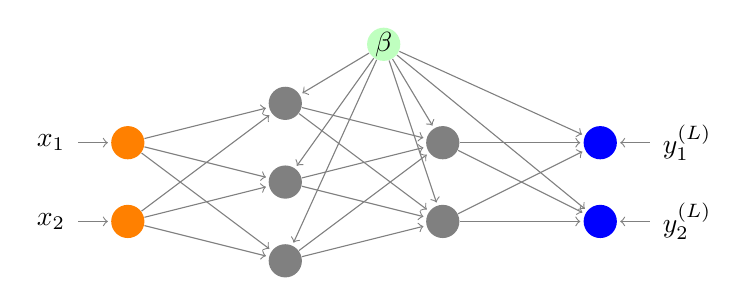
\begin{tikzpicture}[shorten >=1pt,->,draw=black!50, node distance=\layersep]
            \tikzstyle{every pin edge}=[<-,shorten <=1pt]
            \tikzstyle{neuron}=[circle,fill=black!25,minimum size=12pt,inner sep=0pt]
            \tikzstyle{input neuron}=[neuron, fill=orange];
            \tikzstyle{output neuron}=[neuron, fill=blue!100];
            \tikzstyle{hidden neuron}=[neuron, fill=black!50];
            \tikzstyle{annot} = [text width=3em, text centered]

           \node[hidden neuron, fill=green!25] (BIAS) at (3.25,0) {$\beta$};

            % Draw the input layer nodes
            \foreach \name / \y in {1,...,2}
            % This is the same as writing \foreach \name / \y in {1/1,2/2,3/3,4/4}
                \path[yshift=\nodesep]
                    node[input neuron, pin=left: \(x_\y\)] (I-\name) at (0,-0.5 cm -\y  cm) {};

            % Draw the hidden layer nodes
            \foreach \name / \y in {1,...,3}
                \path[yshift=\nodesep]
                    node[hidden neuron] (H1-\name) at (\layersep,-\y) {};

             \foreach \name / \y in {1,...,2}
                \path[yshift=\nodesep]
                    node[hidden neuron] (H2-\name) at (2*\layersep,-0.5cm -\y cm) {};

            % Draw the hidden layer nodes
            \foreach \name / \y in {1,...,2}
                \path[yshift=\nodesep]
                    node[output neuron, pin=right:\(y_{\name}^{(L)}\)] (O-\name) at (3*\layersep,-0.5cm -\y cm) {};


            % Connect every node in the input layer with every node in the
            % hidden layer.
            \foreach \source in {1,...,2}
                \foreach \dest in {1,...,3}
                    \path (I-\source) edge (H1-\dest);

            % Connect every node in the hidden layer with the output layer

            \foreach \source in {1,...,3}
                \foreach \dest in {1,...,2}
                    \path (H1-\source) edge (H2-\dest);
            \foreach \source in {1,...,2}
                \foreach \dest in {1,...,2}
                \path (H2-\source) edge (O-\dest);

              %Connect the bias
                \foreach \dest in {1,...,3}
                    \path (BIAS) edge (H1-\dest);
                \foreach \dest in {1,...,2}
                    \path (BIAS) edge (H2-\dest);
                \foreach \dest in {1,...,2}
                    \path (BIAS) edge (O-\dest);

            % Annotate the layers
        \end{tikzpicture}
        %   \caption[An example of a feed-forward ANN]{An example of a feed-forward ANN,  \(\mathcal{N}\) with four layers.}
        \end{figure}

        \begin{definition}
          A \textbf{weight} on the $\ell$th layer between the $j$th neuron on that layer and
          the $i$th neuron on the next layer is denoted $w^{\ell}_{ij} \in \mathbb{R}.$
        \end{definition}
        \begin{definition}
          The \textbf{input} to the neural network is a vector $\pmb x \in \mathbb{R}^n$ and the
          \textbf{output} is a vector $\pmb y \in \mathbb{R}^m.$
        \end{definition}
    \end{frame}

    \begin{frame}
    \frametitle{A Bit of Notation}
      \begin{figure}
        \centering
            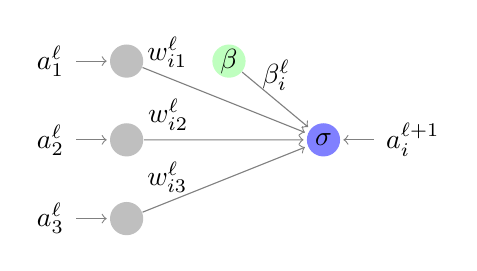
\begin{tikzpicture}[shorten >=1pt,->,draw=black!50, node distance=\layersep]
            \tikzstyle{every pin edge}=[<-,shorten <=1pt]
            \tikzstyle{neuron}=[circle,fill=black!25,minimum size=12pt,inner sep=0pt]
            \tikzstyle{output neuron}=[neuron, fill=blue!50];
            \tikzstyle{annot} = [text width=3em, text centered]

           \node[neuron, fill=green!25] (BIAS) at (1.3,-1.25) {$\beta$};

            % Draw the input layer nodes
            \foreach \name / \y in {1,...,3}
            % This is the same as writing \foreach \name / \y in {1/1,2/2,3/3,4/4}
                \path[yshift=\nodesep]
                    node[neuron, pin=left: \(a_\y^{\ell}\)] (I-\name) at (0,-0.5 cm -\y  cm) {};


                \path[yshift=\nodesep]
                    node[output neuron, pin=right:\(a_i^{\ell+1}\)] (OUTPUT) at (\layersep + 0.5cm,-2.5 cm) {$\sigma$};


            % Connect every node in the input layer with every node in the
            % hidden layer.
            \foreach \source in {1,...,3}
                    \path (I-\source) edge  node [pos=0.15, above]{\(w_{i\source}^\ell \)} (OUTPUT);

              \path (BIAS) edge node [midway, above]{\(\beta_{i}^\ell \)} (OUTPUT);

            % Annotate the layers
        \end{tikzpicture}
      \end{figure}
       \begin{definition}
         The \textbf{output} of the $i$th neuron on the $(\ell+1)$th layer is given by the weighted sum of its inputs
         \[a^{\ell+1}_i = \sigma\left(\sum_{j \in A_i}a_j^{\ell}w_{ij}^\ell + \beta^{\ell}_i\right)\]
         where $A_i$ is the set of anterior neurons.
         \end{definition}

    \end{frame}


    \begin{frame}
      \frametitle{The Sigmoid Activation Function}
      \begin{figure}
          \centering
          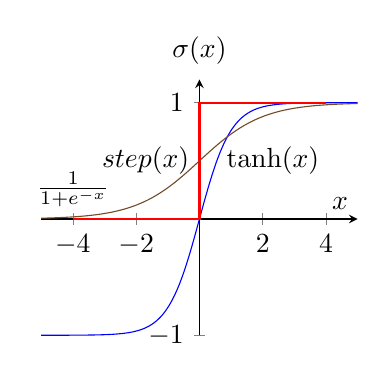
\begin{tikzpicture}
              \begin{axis}[
                axis lines=middle,
                clip=false,
                ymin=-1,
                ymax=1.2,
                ylabel=$\sigma(x)$,
                xlabel=$x$,
                every axis y label/.style={
                    at={(ticklabel* cs:1.02)},
                    anchor=south,
                },
                legend pos=north west,
                width=5.6cm,
                ytick={-1,1}
              ]
              \addplot+[mark=none,samples=200,unbounded coords=jump] {tanh(x)} node[right,pos=.57,black] {$\tanh(x)$};;
              \addplot+[const plot, no marks, thick] coordinates {(-4,0) (0,0) (0,1) (4,1)} node[left,pos=.5,black] {$step(x)$};
              \addplot+[mark=none,samples=200,unbounded coords=jump] {1/(1+exp(-x))} node[above,pos=.1,black] {$\frac{1}{1+e^{-x}}$};;
              \end{axis}
          \end{tikzpicture}

        \caption{Two sigmoid functions and the perceptron $step(x).$}
        \label{fig:test}
        \end{figure}
        \begin{definition}
          We say that $\sigma : \mathbb{R} \to \mathbb{R}$ is a \textbf{sigmoid activation function} if
          $\sigma(x) \to 1 $ as $ x \to \infty$ and $\sigma(x) \to -1\;\text{or}\; 0$ as $ x \to -\infty$

        \end{definition}
    \end{frame}


    \begin{frame}
      \frametitle{The Feed-Forward Algorithm}
       \begin{figure}
        \centering
        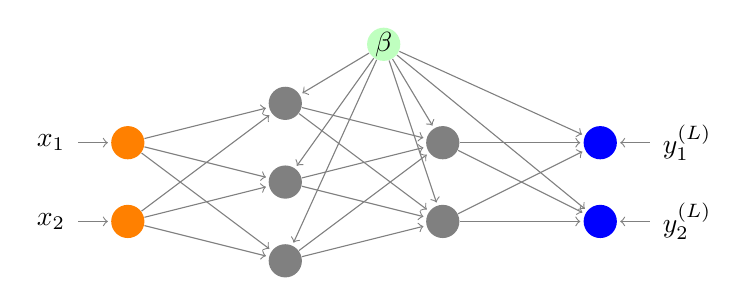
\begin{tikzpicture}[shorten >=1pt,->,draw=black!50, node distance=\layersep]
            \tikzstyle{every pin edge}=[<-,shorten <=1pt]
            \tikzstyle{neuron}=[circle,fill=black!25,minimum size=12pt,inner sep=0pt]
            \tikzstyle{input neuron}=[neuron, fill=orange];
            \tikzstyle{output neuron}=[neuron, fill=blue!100];
            \tikzstyle{hidden neuron}=[neuron, fill=black!50];
            \tikzstyle{annot} = [text width=3em, text centered]

           \node[hidden neuron, fill=green!25] (BIAS) at (3.25,0) {$\beta$};

            % Draw the input layer nodes
            \foreach \name / \y in {1,...,2}
            % This is the same as writing \foreach \name / \y in {1/1,2/2,3/3,4/4}
                \path[yshift=\nodesep]
                    node[input neuron, pin=left: \(x_\y\)] (I-\name) at (0,-0.5 cm -\y  cm) {};

            % Draw the hidden layer nodes
            \foreach \name / \y in {1,...,3}
                \path[yshift=\nodesep]
                    node[hidden neuron] (H1-\name) at (\layersep,-\y) {};

             \foreach \name / \y in {1,...,2}
                \path[yshift=\nodesep]
                    node[hidden neuron] (H2-\name) at (2*\layersep,-0.5cm -\y cm) {};

            % Draw the hidden layer nodes
            \foreach \name / \y in {1,...,2}
                \path[yshift=\nodesep]
                    node[output neuron, pin=right:\(y_{\name}^{(L)}\)] (O-\name) at (3*\layersep,-0.5cm -\y cm) {};


            % Connect every node in the input layer with every node in the
            % hidden layer.
            \foreach \source in {1,...,2}
                \foreach \dest in {1,...,3}
                    \path (I-\source) edge (H1-\dest);

            % Connect every node in the hidden layer with the output layer

            \foreach \source in {1,...,3}
                \foreach \dest in {1,...,2}
                    \path (H1-\source) edge (H2-\dest);
            \foreach \source in {1,...,2}
                \foreach \dest in {1,...,2}
                \path (H2-\source) edge (O-\dest);

              %Connect the bias
                \foreach \dest in {1,...,3}
                    \path (BIAS) edge (H1-\dest);
                \foreach \dest in {1,...,2}
                    \path (BIAS) edge (H2-\dest);
                \foreach \dest in {1,...,2}
                    \path (BIAS) edge (O-\dest);

            % Annotate the layers
        \end{tikzpicture}
        %   \caption[An example of a feed-forward ANN]{An example of a feed-forward ANN,  \(\mathcal{N}\) with four layers.}
        \end{figure}
        \begin{itemize}
          \item The feed-forward algorithm propagates input through the neural network
          layer by layer.
          \item On every layer each neuron accumulates input from previous layers
          and then \emph{activates} through the sigmoid activation function.
        \end{itemize}
    \end{frame}


    \begin{frame}
      \frametitle{The Feed-Forward Algorithm}

        \begin{figure}
        \centering
            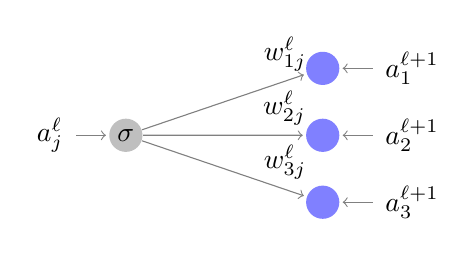
\begin{tikzpicture}[shorten >=1pt,->,draw=black!50, node distance=\layersep]
            \tikzstyle{every pin edge}=[<-,shorten <=1pt]
            \tikzstyle{neuron}=[circle,fill=black!25,minimum size=12pt,inner sep=0pt]
            \tikzstyle{output neuron}=[neuron, fill=blue!50];
            \tikzstyle{annot} = [text width=3em, text centered]

            % Draw the input layer nodes
            \foreach \name / \y in {2}
            % This is the same as writing \foreach \name / \y in {1/1,2/2,3/3,4/4}
                \path[yshift=\nodesep]
                    node[neuron, pin=left: \(a_j^{\ell}\)] (INPUT) at (0,-0.5 cm -\y  cm) {$\sigma$};

            \foreach \name / \y in {1,...,3}
                \path[yshift=\nodesep]
                    node[output neuron, pin=right:\(a_\name^{\ell+1}\)] (O-\name) at (\layersep + 0.5cm,-0.5cm -0.85*\y cm - 0.3cm ) {};


            % Connect every node in the input layer with every node in the
            % hidden layer.
            \foreach \source in {1,...,3}
                    \path (INPUT) edge  node [pos=0.87,above]{\(w_{\source j}^\ell \)} (O-\source);

            % Annotate the layers
        \end{tikzpicture}
      \end{figure}

\begin{algorithm}[H]
\begin{algorithmic}[1]
\FOR{layer $\ell=1$ to $L-1$}
\FOR{neuron $a_j$ on layer $\ell$}
\STATE $a_j.activate()$\
\FOR{neuron $a_i$ on layer $\ell+1$}
\STATE $a_i.feed(w_{ij} a_j)$\
\ENDFOR
\ENDFOR
\ENDFOR
\end{algorithmic}
\caption{An Intuitive Version}

\end{algorithm}
    \end{frame}



%------------------------------------------------
\subsection{An Implementation}
\begin{frame}
\frametitle{Our Network Implementation}
\begin{block}{Network}
    \begin{itemize}
        \item List of neurons and List of connections
        \item Feedforward Method
        \item Backpropagation Method
    \end{itemize}
% The network class will contain all of the network construction logic and the primary network methods. It will contain a list that contains all of the neurons, a list that contains all of the connections, a method for feedforward, and a method for backpropagation.
\end{block}

\begin{block}{Neuron}
    \begin{itemize}
        \item List of connections anterior and posterior connections
        \item Feed Method
        \item Activation Method
        \item Error update
    \end{itemize}
\end{block}
\end{frame}

%------------------------------------------------

\begin{frame}
\frametitle{Our Network Implementation}
\begin{block}{Connection}
    General weight information
    \begin{itemize}
        \item Reference to anterior and posterior neuron
        \item Weight value
        \item Feedforward
    \end{itemize}
\end{block}
\end{frame}
\section{Training}
\begin{frame}
    \frametitle{Training}
    \begin{itemize}
        \item The goal of machine learning is to adjust learning parameters to better approximate a function.
        \item For neural networks, these learning parameters are the weights and the bias values.
        \item We train our network by trying to minimize a loss function:  $$E = \sum (\delta_{i}-y_{i})^2$$ where $\delta$ is the expected output and $y$ is the actual output.
        \item Minimizing the loss function is a nonconvex problem - we need to develop heuristics to properly train the network
        \item One such heuristic is called gradient descent
    \end{itemize}
\end{frame}


\subsection{Nonconvex Optimization}


\begin{frame}
    \frametitle{Gradient Descent and Error Backpropagation (Calculus Heavy)}
    \begin{center}
        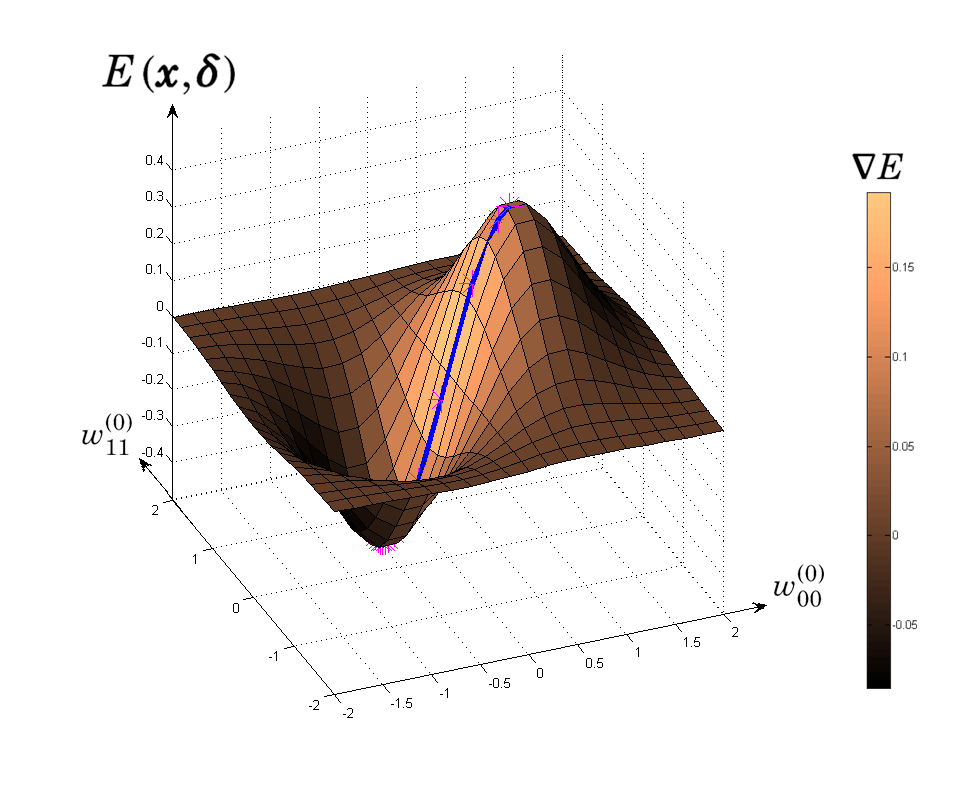
\includegraphics[width=0.5\textwidth]{gradient_descent}
    \end{center}
    \begin{itemize}
        \item The goal is to travel down the gradient (slope at a point)
         towards a minima of the error function.
        \item Error backpropagation is an algorithm that calculates the gradient
        and then updates the weights according to a \emph{learning rate.}
    \end{itemize}
\end{frame}

\begin{frame}
    \begin{definition}
    We call \(\pmb{\nabla}E\) the \textbf{gradient} of \(E\) if 
    \[\pmb{\nabla}E = \left(\frac{\partial E}{\partial w_{00}^{(0)}}, 
    \frac{\partial E}{\partial w_{01}^{(0)}},\dots,
    \frac{\partial E}{\partial w_{ij}^{(L)}}\right).\]
    \end{definition}

    \begin{algorithm}[H]
    \begin{algorithmic}[1]
    \FOR{every weight $w_{ij}^\ell$}
    \STATE calculate $\Delta w_{ij}^\ell = -\alpha \frac{\partial E}{\partial w_{ij}^\ell}$ \
    \STATE $w^\ell_{ij} + \Delta w_{ij}^\ell \to w_{ij}^\ell$ \
    \ENDFOR
    \end{algorithmic}
    \caption{The Weight Update Rule}

    \end{algorithm}
\end{frame}




\subsection{Training Demo}
\begin{frame}[fragile]
    \frametitle{Program Reference}
    \begin{example}[Creating a network, loading a dataset, and training the net]
        \verbatimfont{\scriptsize}
        \begin{verbatim}
n = Network(<list of layer sizes>)
t = Trainer(n)
t.load_data(<string of the filename>)
t.interactive_step(<learning_rate> [, optional verbose flag])
        \end{verbatim}
    \end{example}
  \begin{example}[A dataset file]
        \verbatimfont{\scriptsize}
        \begin{verbatim}
# This is a sample data file
# You can comment with ####
# This dataset has two inputs and one desired output
{0,1} -> {1};
{1,0} -> {1};
{0,0} -> {0.3};
        \end{verbatim}
    \end{example}
\end{frame}
\section{Deep Learning}
\begin{frame}
    \frametitle{Deep Learning}
    \begin{center}
        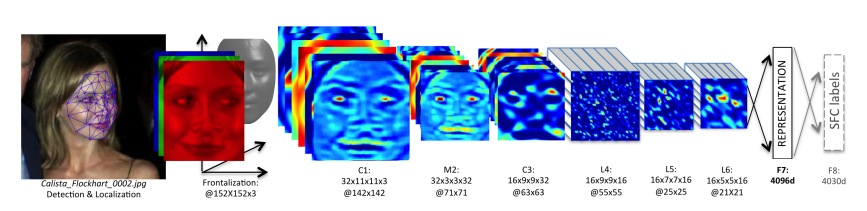
\includegraphics[scale=.34]{deepfaces}
    \end{center}
    \begin{itemize}

        \item A more powerful variation of the artificial neural network that uses deep architecture, where there are many hidden layers in a network
        \item Represnts problems as a heirarchy of concepts and representations
        \item Each concept is defined in relation to simpler concepts.
    \end{itemize}
\end{frame}
\begin{frame}
    \frametitle{Deep Learning}
    \begin{itemize}
        \item Neural networks saw a number of falls from popularity
        \item Two main events occurred that brought neural networks back
        \begin{itemize}
            \item The availability of better hardware and more extensive dataset (think big data)
            \item The creation of more simplified training methods for deep network architectures
        \end{itemize}
        \item With the availability of better hardware and large datasets (think big data
    \end{itemize}
\end{frame}

\begin{frame}
\frametitle{References}
\footnotesize{
\begin{thebibliography}{99} % Beamer does not support BibTeX so references must be inserted manually as below
\bibitem[Smith, 2012]{p1} John Smith (2012)
\newblock Title of the publication
\newblock \emph{Journal Name} 12(3), 45 -- 678.
\end{thebibliography}
}
\end{frame}

%------------------------------------------------

\begin{frame}
\Huge{\centerline{The End}}
\end{frame}

%----------------------------------------------------------------------------------------

\end{document}
